\documentclass[../mit-general-chemistry.tex]{subfiles}
\begin{document}

\chapter{Atomic theory}

J.~J.~Thomson is commonly cited as the discoverer of the
electron. Although other contemporary scientists als suggested that
atoms were composed of even smaller components, Thomson was the first
to suggest the idea of the electron -- a particle more than a thousand
times smaller than the atom itself.

Thomson, at the time, studied cathode rays and doing so discovered
that they traveled further through air than an atom sized particle
would and this made him suggest that the rays consisted of particles a
thousand the size of atoms. He also observed that the particles, which
he called {\em corpuscles}, were negatively charged and had the same
mass, no matter which sort of atom they came from. Later scientists
preferred the particles named electrons.

Thomson's first experiment, as it is called, showed that he could
deflect the cathode ray using electromagnets. Thomson concluded that
this proved that the negative charge and the ray were inseparable and
intertwined.

In his second experiment, Thomson deflected the cathode ray by
applying an electric field between two metal plates. This allowed
Thomson to prove, beyond a shadow of a doubt, that the ray consisted
of negatively charged particles.

In the third experiment, Thomson used varying currents to deflect the
ray. This gave him a measurement of the charge to mass ratio. The
large number faced him with a conundrum: did the large number mean
that the particles carries a huge charge or were they incredible
small? Thomson was convinced on the latter and postulated that the
particles emanated from within the atoms themselves.

Thomson that all atoms consisted of a diffuse cloud of positive charge
with the electrons embedded within it. This is called the plum pudding
model.

In 1908, Robert Millikam performed experiments with charged oil
drops. In an apparatus he let tiny, charged oil drops fall inside a
box. The fall of the oil drops can be controlled by applying current
to two metal plates inside the box. This let Millikam estimate the
magnitude of charge of the electron (?). From this, he could use the
charge to mass ratio from Thomson's experiments to decide the mass of
the electron.

In 1911, Ernest Rutherford, in his gold foil experiment, set up an
experiment in which $\alpha$-particles where to pass through a foil of
gold. This would be in line with Thomson's theories. The gold foil was
surrounded wuth a fluorescing detector screen with a slit to allow the
$\alpha$-particles to enter the detector. Surprisingly, Rutherford
detected that most of the particles indeed passed straight through the
foil, some were slightly deflected. There were, however, a small
number of $\alpha$-particles that were back scattered and even some
that bounced back out of the detector. This was not in accordance with
the model of the plum pudding. Rutherford concluded that the
scattering $\alpha$-particles had hit a concentrated positively
charged center of the atom containing most of it's mass. The finds
were explained by a new model of the nuclear atom with the positive
nucleus surrounded by orbiting electrons.



\section{Wave-particle duality of light}

Newtonian mechanics does not work on atomic and subatomic scale.

Quantum mechanics takes the wave-particle duality into account. Light
consists of discrete packets of energy called photons.


\subsection{Properties of waves}


Waves have periodic variation of some quantity. For the waves in the
sea the varying quantity is the sea level. The waves have high, low
and average levels.

In the case of sound waves the varying property is density and the
variation is between high and low density.


\begin{hfigure}
  \begin{center}
    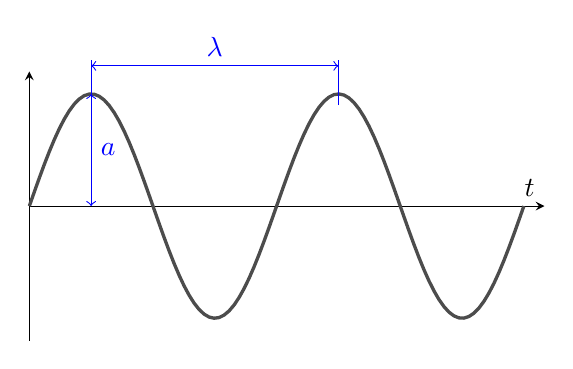
\begin{tikzpicture}
      \begin{axis}[
          axis lines=middle,
          width=.67\textwidth,
          height=5cm,
          axis lines = middle,
          domain = 0:720,
          ymin=-1.2,
          ymax=1.2,
          xmax=750,
          xtick=\empty,
          ytick=\empty,
          xlabel=$t$,
          clip = false
        ]
        \addplot[black!70, very thick, samples=100]{sin(x)};
        \draw [blue](90, .9) -- (90, 1.3);
        \draw [blue](450, .9) -- (450, 1.3);
        \draw [<->, blue](90, 1.25) -- (450, 1.25) node[midway,above]{$\lambda$};
        \draw [<->, blue](90, 0) -- (90, 1) node[midway,right]{$a$};
      \end{axis}
    \end{tikzpicture}%
  \end{center}
  \caption{Basic properties of waves.}
\end{hfigure}



Mathematically, waves have periodicity/frequency and amplitude.
\begin{equation}
  f = \frac{v}{\lambda}\quad v \text{~is the speed of the wave}
\end{equation}
\begin{equation}
  f = \frac{cycles}{\Delta t}
\end{equation}


Light (electromagnetic radiation) is a periodic variation of an
electric field.

An electric field is a space through which Coulomb force operates.


\begin{equation}
  E(x, t) = a\cdot\cos \left[ 2\pi \left( \frac{x}{\lambda} - \nu t \right) \right]
\end{equation}

where $E$ is the electric field, $x$ the position of the wave, $\nu$
the frequency of the wave and $t$ the time.

If we want to study the wave one trick is to keep one of the variables
constant and study the result. If we hold the time constant, we can
visualize the electric field as a function of the position, $x$.

\begin{equation}
  E(x, 0) = a\cdot\cos \left[ \frac{2\pi x}{\lambda}  \right]
\end{equation}

Also, as $a$ is the amplitude $a^2 = intensity$ of wave.



We can also keep $x$ constant, e.g. $x = 0$ and consider the equation
as a function of $t$ only 
\begin{equation}
  E(0, t) = a\cdot\cos \left[ 2\pi\nu t \right]
\end{equation}

$E(t) = 1$ when $t = \frac{n}{\nu}$ for $n\in\mathbb{Z}$.

\begin{equation}
  \frac{1}{\nu} = period
\end{equation}

Period of a wave is the time it takes for one cycle to occur.

Units of frequency ($\nu$) is almost always number of cycles per
second= Hz (i.e. $\SI{5}{\per\second} = 5$ Hz).

The speed of a wave can be expressed as how long time it takes for a
wave to travel one wavelength. It is going to take one period to move
that distance ($\Delta t = \frac{1}{\nu}$).

So
\begin{equation}
  speed = \frac{\lambda}{\frac{1}{\nu}} = \lambda \nu~\si{\meter\per\second}
\end{equation}

Electromagnetic radiation has constant speed. The speed of light

\begin{equation}
  c = \lambda \nu = \SI{299792458}{\meter\per\second}
\end{equation}



\subsection{Superposition of waves: In phase superposition: Constructive interference}


\begin{hfigure}
  \begin{center}
    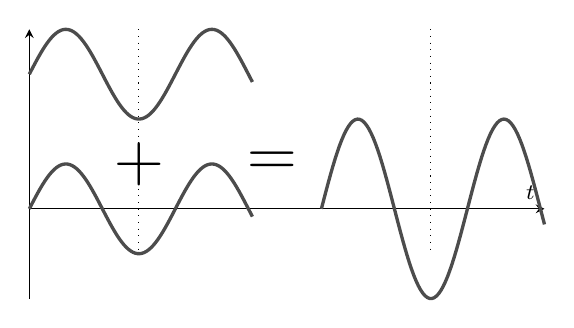
\begin{tikzpicture}[
        >=latex,
        font={\footnotesize},
        declare function={
          f(\x) = sin(\x);
        }
      ]
      \begin{axis}[
          axis lines=middle,
          width=.67\textwidth,
          height=5cm,
          axis lines = middle,
          domain = 0:720,
          xtick=\empty,
          ytick=\empty,
          xlabel=$t$,
          clip = false
        ]
        \addplot[domain=0:550,black!70, very thick, samples=100]{sin(x)};
        \addplot[domain=0:550,black!70, very thick, samples=100]{3 + sin(x)};
        \addplot[domain=720:1270,black!70, very thick, samples=100]{2*sin(x)};
        \draw [dotted] (270, 4) -- (270, -1);
        \draw [dotted] (990, 4) -- (990, -1);
        \node at (270, 1){{\Huge +}};
        \node at (600, 1){{\Huge =}};
      \end{axis}
    \end{tikzpicture}%
  \end{center}
  \caption{Constructive interference.}
\end{hfigure}



\subsection{Destructive interference}


\begin{hfigure}
  \begin{center}
    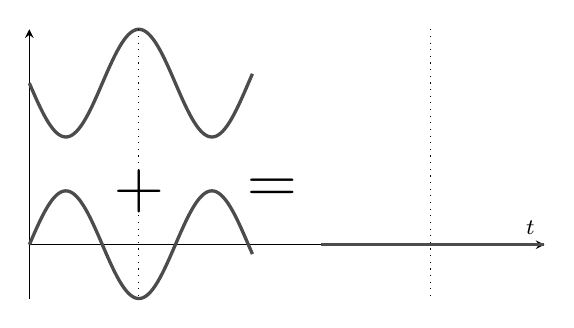
\begin{tikzpicture}[
        >=latex,
        font={\footnotesize},
        declare function={
          f(\x) = sin(\x);
        }
      ]
      \begin{axis}[
          axis lines=middle,
          width=.67\textwidth,
          height=5cm,
          axis lines = middle,
          domain = 0:720,
          xtick=\empty,
          ytick=\empty,
          xlabel=$t$,
          clip = false
        ]
        \addplot[domain=0:550,black!70, very thick, samples=100]{sin(x)};
        \addplot[domain=0:550,black!70, very thick, samples=100]{3 + sin(x + 180)};
        \addplot[domain=720:1270,black!70, very thick, samples=100]{0};
        \draw [dotted] (270, 4) -- (270, -1);
        \draw [dotted] (990, 4) -- (990, -1);
        \node at (270, 1){{\Huge +}};
        \node at (600, 1){{\Huge =}};
      \end{axis}
    \end{tikzpicture}%
  \end{center}
  \caption{Destructive interference.}
\end{hfigure}



\section{Light as particles}


WHat are the wave properties observed of light? What are the particle
properties observed?



\subsection{Photoelectric effect}

Pick any metal and shine a UV-light on it. If the frequency ($\nu$) of
the UV-light is above the threshold frequency of that specific metal
electrons are emitted from the metal.


\begin{hfigure}
  \begin{center}
    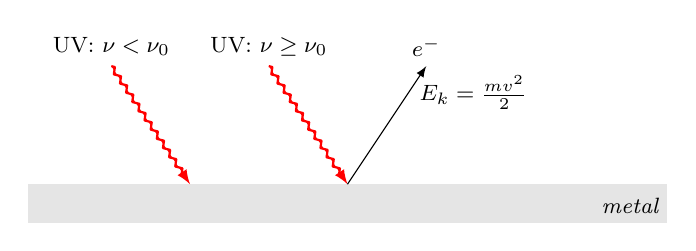
\begin{tikzpicture}[
        >=latex,
        font={\footnotesize}
      ]
      \node (rect) [
        rectangle,
        %draw=black!40,
        fill=black!10,
        minimum width=.67\textwidth,
        minimum height=5mm,
        anchor= south, label={[anchor=south east]south east:{\em metal}}
      ] at (0,0) {};    
      \draw [
        ->,
        draw=red,
        fill=red,
        thick,
        >=latex,
        line join=round,
        decorate, decoration={
          zigzag,
          segment length=4,
          amplitude=.9,post=lineto,
          post length=2pt,
      }]  (-3, 2cm) -- (-2, 5mm)
      node [at start,above] {UV: $\nu < \nu_0$};
      \draw [
        ->,
        draw=red,
        fill=red,
        thick,
        >=latex,
        line join=round,
        decorate, decoration={
          zigzag,
          segment length=4,
          amplitude=.9,post=lineto,
          post length=2pt,
      }]  (-1, 2cm) -- (0, 5mm)
      node [at start,above] {UV: $\nu \geq \nu_0$};
      \draw[->](0, 5mm) -- (1, 2cm) node[at end,above]{$e^-$}
      node[at end, below,xshift=6mm]{$E_k = \frac{mv^2}{2}$};
    \end{tikzpicture}
  \end{center}
  \caption{The photoelectric effect. When irradiating a metal with
    high enough energy light an electron is emitted. }
\end{hfigure}

Making a diagram for numbers of electrons ejected for different
frequencies was disturbing,


\begin{hfigure}
  \hspace*{\fill}
  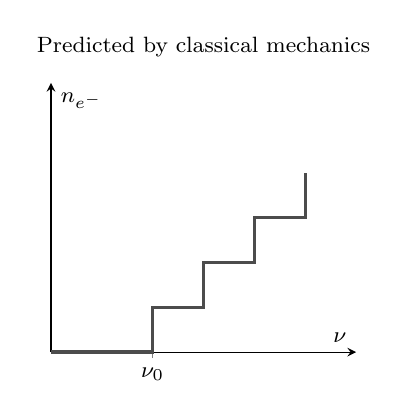
\begin{tikzpicture}[
      >=latex,
      font={\footnotesize},
      declare function={
        f(\x) = sin(\x);
      }
    ]
    \begin{axis}[
        axis lines=middle,
        width=.45\textwidth,
        height=5cm,
        axis lines = middle,
        domain = 0:5,
        xmin=0,
        xmax=6,
        ymin=0,
        ymax=6,
        xtick={2},
        xticklabels={$\nu_0$},
        ytick={0},
        yticklabels={0},
        title={Predicted by classical mechanics},
        xlabel=$\nu$,
        ylabel=$n_{e^-}$,
        clip = false
      ]
      \draw[black!70, very thick]
      (0, 0) --
      (2, 0) -- (2, 1) --
      (3, 1) -- (3, 2) --
      (4, 2) -- (4, 3) --
      (5, 3) -- (5, 4);
    \end{axis}
  \end{tikzpicture}%
  \hfill%
  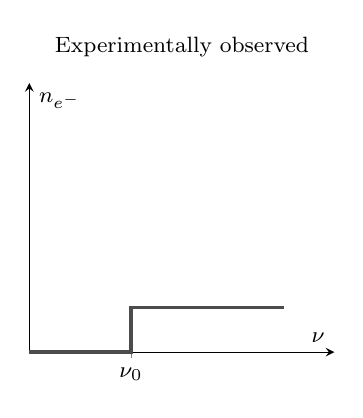
\begin{tikzpicture}[
      >=latex,
      font={\footnotesize},
      declare function={
        f(\x) = sin(\x);
      }
    ]
    \begin{axis}[
        axis lines=middle,
        width=.45\textwidth,
        height=5cm,
        axis lines = middle,
        domain = 0:5,
        xmin=0,
        xmax=6,
        ymin=0,
        ymax=6,
        xtick={2},
        xticklabels={$\nu_0$},
        ytick={0},
        yticklabels={0},
        title={Experimentally observed},
        xlabel=$\nu$,
        ylabel=$n_{e^-}$,
        clip = false
      ]
      \draw[black!70, very thick] (0, 0) -- (2, 0) -- (2, 1) -- (5, 1);
    \end{axis}
  \end{tikzpicture}%
  \hspace*{\fill}
  \caption{
  Scientists predicted that the number of emitted electrons from the
  photoelectric effect would be showing a linear dependency on the
  frequency (energy) of light, but experiments failed to show that.
  }
\end{hfigure}


Scientists were puzzled since they expected the number of ejected
electrons to rise with the frequency.

... all the failed predictions of the electron's kinetic energy made
by scientists


\subsubsection{A new model of the photoelectric effect}



\begin{center}
  \begin{tikzpicture}[
      >=latex,
      font={\footnotesize},
      declare function={
        f(\x) = sin(\x);
      }
    ]
    \begin{axis}[
        axis lines=middle,
        width=.67\textwidth,
        height=5cm,
        axis lines = middle,
        hide x axis,
        domain = 0:10,
        xmin=0,
        xmax=10,
        ymin=0,
        ymax=10,
        xtick=\empty,
        ytick={5},
        yticklabels={$E_{e^-}$},
        title={New model of the photoelectric effect},
        xlabel=$\nu$,
        ylabel=$E$,
        clip = false
      ]
      \draw[dashed] (0, 5) -- (10, 5);

      \draw (1, 2) -- (2, 2);
      \draw [<->](1.5, 2) -- (1.5, 5) node[midway, right]{$\phi = hv_0$};

      \draw (4, 2) -- (5, 2);
      \draw (4, 8) -- (5, 8);
      \draw [<->](4.5, 2) -- (4.5, 8) node[midway, right, yshift=2mm]{$E_i = hv$};

      \draw (7, 8) -- (8, 8);
      \draw [<->](7.5, 5) -- (7.5, 8) node[midway, right]{$E_k$};
    \end{axis}
  \end{tikzpicture}%
\end{center}


where $E_{e^-}$ is the energi of a free electron; $h$ is Planck's
constant $6.626\times 10^{-34}$ \si{\joule\second}; $E_i = hv$ is the
energy of the incident photon; $\phi = hv_0$ is the work function (the
required energy to get metal to eject electron) and $E_k$ is the
kinetic energy of the ejected electron.



Interpret these:

\begin{equation}
  E_k = E_i - \phi
\end{equation}

\begin{equation}
  E_i = E_k + \phi
\end{equation}





\section{Wave-particle duality of matter, Schrödinger equation}


In problems, {\em photons} may be referred to as light or
electromagnetic radiation. Photons may be described in energy,
$\lambda$ or $\nu$.

{\em Electrons} may be called photoelectrons and are described by
kinetic energy ($E_k$), velocity ($v$) or wavelength ($\lambda$).

{\em electron volt} ($eV$) is a unit of energy: $1.6022\times
10^{-19}$ \si{\joule}.


\begin{example}[In class photoelectric effect demonstration]
  Using Zinc (\ce{Zn}) with $\phi_{\ce{Zn}} = 6.9 \times 10^{-19}$
  \si{\joule}, we're going to use two light sources

  \begin{center}
    \begin{tabular}{ll}
      UV-light (U) & $\lambda = \SI{254}{\nano\meter}$ \\
      Red laser pointer (L) & $\lambda = \SI{700}{\nano\meter}$ \\
    \end{tabular}
  \end{center}

  Consider three questions

  \begin{enumerate}
  \item What is the energy emitted per photon emitted by the UV lamp?
  \item What is the energy emitted per photon emitted by the laser
    pointer?
  \item What is the total number of photons emitted by the laser
    pointer in \SI{60}{\second} if the intensity $I =
    \SI{1}{\milli\watt}$?
  \end{enumerate}

  Remember that speed of light, $c =
  \SI{299792458}{\meter\per\second}$ and that $speed = \nu\lambda$.

  \textbf{Solution}

  We know that $E = h\nu$ and that $\nu = \frac{c}{\lambda}$ so
  \begin{equation}
    E = \frac{hc}{\lambda} = \frac{6.6022\times 10^{-34} \cdot
      299792458}{\lambda} = \frac{1.986\times 10^{-25}}{\lambda}
  \end{equation}
  for each of the light sources so

  \begin{align*}
    E_U &= \frac{1.986\times 10^{-25}}{\lambda} =
    \frac{1.986\times 10^{-25}}{254\times 10^{-9}} =
    7.821\times 10^{-19} \si{\joule} \\
    E_L &= \frac{1.986\times 10^{-25}}{\lambda} =
    \frac{1.986\times 10^{-25}}{700\times 10^{-9}} =
    2.84\times 10^{-19} \si{\joule} \\
  \end{align*}

  Which means that $E_U > \phi_{\ce{Zn}}$ and that $E_L <
  \phi_{\ce{Zn}}$ so we predict that using the UV lamp we should be
  able to make the zinc plate emit electrons. Using the laser pointer
  will not. Which answers question (1) and (2).

  Number of photons emitted from the laser pointer during
  \SI{60}{\second} is calculated from

  (3): saying that the effect of the laser pointer is 1 mW just means
  that it is \SI{1}{\joule\per\second} which we can use and write
  \begin{equation*}
    \frac{1.00\times 10^{-3}}{\si{\second}}
    \cdot \frac{(photons)}{2.84\times 10^{-19} \si{\joule}}
    \cdot \SI{60}{\second} =
    2.1\times 10^{17} \text{protons}
  \end{equation*}

  Even though this is a huge number it will not make the zinc plate
  eject any electrons which tells us that this is not a factor in the
  photoelectric effect.
\end{example}


\subsubsection{Photon momentum}

As photons appear to have particle like properties, do they also have
momentum. Photons do not have mass so we can not use $p = mv$. Albert
Einstein proposed a new equation 

\begin{definition}[Photon momentum]
  Since photons have no mass, we need a special definition for the
  photon momentum. Albert Einstein put forth this one
  \begin{align*}
    p &= \frac{h\nu}{c} \implies
    p = \frac{h}{\lambda}
    \quad\text{since}~c = \nu\lambda \\
  \end{align*}
\end{definition}


This was supported by experimental observation. Compton shot X-ray
light at a stationary electron and observed that the electron
scattered as if the momentum of the photons were being
transferred. This would suggest particle like properties of light, of
photons.



\begin{hfigure}
  \begin{center}
    \begin{tikzpicture}
      \coordinate(atelec1) at (0, 0);
      \coordinate(northeast) at (30:2cm);
      \coordinate(west) at (180:2cm);
      \coordinate(southeast) at (330:2cm);
      \node[electron] (elec1) at (atelec1) {$e$};
      \node[electron] (elec2) at (southeast) {$e$};
      \draw [radiation]  (west) -- (elec1.west);
      \draw [radiation]  (elec1.north east) -- (northeast);
      \draw[->, thick] (elec1.south east) -- (elec2.north west);
    \end{tikzpicture}
  \end{center}
  \caption{
    Electrons exposed to X-ray light scattered as if the momentum of
    the X-ray photons where transferred to the electrons. This
    suggested particle like properties of the photons.
  }
\end{hfigure}



\subsubsection{Louis de Broglie}

Einstein says that light is particle-like sometimes. Light has a
wavelength and if it has a wavelength we say it can have
momentum. Louis de Broglie: If light who has a wavelength can have
momentum --- then it must also be true that matter, who has momentum
has a wavelength.

\begin{equation}
  p = \frac{h}{\lambda} \implies \lambda = \frac{h}{p}
\end{equation}

or in another way

Since $p = mv$ $\lambda = \frac{h}{mv}$.

Why do we not observe wave-like behavior of ordinary objects in daily
life? We understand it if we calculate the wavelength large objects,
even extremely fast ones, we see that they are undetectable small
(basbeball att 42 m/s $\lambda = 1.1\cdot 10^{-31} \si{\meter}$),
which make the wave-like behavior unnoticeable.



\begin{example}
  Consider the wavelength of a gaseous electron traveling at
  \SI{1d5}{\meter\per\second}.

  \begin{tabular}{ll}
    $h$ & \SI{6.626d-34}{\second\meter\kilogram\per\square\second} \\
    $m_{electron}$ & \SI{9d-31}{\kilogram} \\
    $v$ & \SI{1d5}{\meter\per\second} \\
  \end{tabular}

  Plug it into the equation

  \begin{equation*}
    \lambda = \frac{h}{mv} = \frac{\SI{6.626d-34}{\second\meter\kilogram\per\square\second}}{(\SI{9d-31}{\kilogram})(\SI{1d5}{\meter\per\second})}
    = \SI{7d-9}{\meter} = \SI{70}{\angstrom}
  \end{equation*}
  
\end{example}

Compare the size of the wavelengths to their environments. The
baseball is ``infinitely'' larger than the calculated wavelength
whereas even an atom is much smaller than the calculated electron
wavelength which is why the wave-like behavior is noticeable from the
electron and not the baseball.




\section{Schrodinger equation}

The Schrodinger equation is an equation of motion which describes
particle by describing it as a wave.

\begin{definition}[Schrodinger equation]
  \begin{equation}
    \hat{H}\Psi = E\Psi
  \end{equation}

  where $\Psi$ is a wave function; $E$ is (in our case) the binding
  energy of the electron to the nucleus; $\hat{H}$ is the Hamiltonian
  operator.

  \begin{equation*}
    \Psi(r, \Theta, \Phi) \quad\text{uses polar coordinates.}
  \end{equation*}

  $r$ is the distance from the nucleus; $\Theta$ is the angle from the
  normal to the $xy$-plane; $\Phi$ is the angle in the $xy$-plane from
  the $x$-axis.

  Now we rewrite the equation

  \begin{equation}
    \hat{H}\Psi(r, \Theta, \Phi) = E\cdot \Psi(r, \Theta, \Phi)
  \end{equation}
\end{definition}


\begin{remark}
  The easiest example of the Hamiltonian operator is the one of the
  hydrogen atom with one electron.

  {\footnotesize
    \begin{equation}
      \hat{H} =
      -\frac{\hslash^2}{m_e}
      \left(
      \frac{1}{r^2}
      \frac{d}{dr}
      \left[
        r^2\frac{d}{dr}
        \right]
      + \frac{1}{r^2\sin\Theta}\frac{d}{d\Theta}
      \left[
        \sin\Theta\frac{d}{d\Theta}
        \right]
      +\frac{1}{r^2\sin\Theta}\frac{d^2}{d\Phi^2}
      \right)
      + U(r)
    \end{equation}
  }

  where $\hslash$ is Planck's redundant constant $\hslash = \frac{h}{2\pi}$.

\end{remark}








\section{The hydrogen atom}



\subsection{Binding energy for the electron to the nucleus}

When we solve the Schrodinger equation
\begin{equation}
  \hat{H}\Psi = E \Psi
\end{equation}
we either solve it to find $\Psi$ which gives us wave functions,
i.e. orbitals; or we solve it to find $E$, the binding energies of the
electron to the nucleus.

For a hydrogen atom
\begin{align*}
  \hat{H}\Psi &= E \Psi \\
  \hat{H}\Psi &= -\frac{1}{n^2}\frac{me^4}{8\epsilon_0^2h^2} \cdot \Psi \\
\end{align*}
where $\epsilon_0$ is permittivity constant, a conversion constant;
$h$ is Plank's constant; $m = m_e$ is the electron mass; $e$ is the
charge on the electron;

This is interpreted as

\begin{equation}
  E = -\frac{1}{n^2}\frac{me^4}{8\epsilon_0^2h^2}
\end{equation}

where $E$ is the binding energy for the electron to the nucleus.

\begin{definition}[The Rydberg constant]
  For convenience we define the Rydberg constant
  \begin{equation}
    \frac{me^4}{8\epsilon_0^2h^2} = R_H = \SI{2.18d-18}{\joule}
  \end{equation}
\end{definition}

Which we can use as such
\begin{equation}
  E_n = -\frac{1}{n^2}\frac{me^4}{8\epsilon_0^2h^2}  = -\frac{R_H}{n^2}
\end{equation}
for the principal quantum number $n = \mathbb{Z}^+$ (positive
integers).

We have that $\lim_{n\to\infty} E_n = 0$ and as this happens we have a
free electron when the binding energy becomes infinitely small. 

As we can see below in the diagram over the first few energy levels of
the hydrogen atom, the gap between energy levels decrease with the
distance to the nucleus.

\begin{hfigure}
  \begin{center}
    \begin{tikzpicture}[
        declare function={
          f(\x) = -(2.18E-18) / \i^2;
        }
      ]
      \begin{axis}[
          title={First energy levels of the hydrogen atom},
          ylabel={$E$},
          width=.8\textwidth,
          height=7cm,
          axis lines = middle,
          hide x axis,
          domain = 2:8,
          ymin=-2.3E-18,
          ymax=0,
          xmin=0,
          xmax=10,
          %ytick = {0},
          clip = false
        ]
        \foreach \i in {1, 2,...,6}{
          \edef\temp{
            \noexpand\addplot [blue,ultra thin]{f(\i)};
          }
          \temp
        }
      \end{axis}
    \end{tikzpicture}%
  \end{center}
  \caption{
    First energy levels of the hydrogen atom from the Schrodinger
    equation.
  }
\end{hfigure}

Energy levels are negative. Lower energy leves yield more stable state
for the atom. The lowest state ($E = R_H$) is called the ground
state. That is the most negative and most stable energy level that we
have.

We can think of the binding energy as the {\em negative of the
  ionization energy} for an hydrogen atom in the $n^{th}$ state.

\begin{equation}
  IE = -E_{n=1}
\end{equation}

When $n = 2$ we talk about {\em the first excited state}. The second
excited state is $n = 3$, the third is $n = 4$ et cetera.


The extended equation
\begin{equation}
  E_n = \frac{Z^2R_H}{n^2}
\end{equation}
correctly predicts the energy levels of any one-electron atom
(hydrogen atoms and ions).

\begin{center}
  \begin{tabular}{lll}
    \ce{H} & 1 $e^-$ atom & $Z = 1$ \\
    \ce{He^+} & 1 $e^-$ atom & $Z = 2$ \\
    \ce{Li^2+} & 1 $e^-$ atom & $Z = 3$ \\
    \ce{Tb^64+} & 1 $e^-$ atom & $Z = 65$ \\
  \end{tabular}
\end{center}

Why?

The Coulomb potential energy between the electron and the nucleus.
\begin{equation}
  U(r) = - \frac{(Ze)e}{4\pi\epsilon_0 r}
\end{equation}
from the solution to the Schrodinger equation for the hydrogen atom
above. In teh equation $Z$ is the number of protons in the nucleus;
$e$ os the number of electrons (?) and the rest is as above. In the
case of the \ce{H} atom $Z = e = 1$ and the nominator becomes 1.

This allow us to calculate the binding energy for all sorts of atoms
given the condition that it have only one electron.








\subsection{Verification of hydrogen atom energy levels}




\subsubsection{Hydrogen atom emission}

If we have a evacuated glass tube with hydrogen gas, the atoms will
become so scarce that we in fact separate the from each other. If we
also have two electrodes in each end of the tube and apply an
electrical potential over the tube we can excite the electrons of the
atoms. As previously excited electrons return to the ground state, we
can observe photons (light) being emitted as the electrons release
energy when they return to the ground state.


\begin{remark}
  Relaxation of an excited hydrogen atom occurs as a previously
  excited electron releases energy as a photon when it leaves an
  excited state and returns to a lower state.

  The energy released is the exact same amount of the energy
  difference between the higher and lower state.
\end{remark}


We can convert between $E$, $\nu$ and $\lambda$ using our previously
defined equations

\begin{align*}
  \nu &= \frac{\deltaE}{h} = \frac{E_{initial} - E_{final}}{h}\\
\end{align*}


Relationship of $E, \nu$ and $\lambda$.




\begin{hfigure}
  \begin{center}
    \begin{tikzpicture}[
        declare function={
          f(\x) = -(2.18E-18) / \i^2;
        }
      ]
      \begin{axis}[
          %title={First energy levels of the hydrogen atom},
          ylabel={$E$},
          width=.67\textwidth,
          height=7cm,
          axis lines = middle,
          hide x axis,
          domain = 0:10,
          ymin=0,
          ymax=6,
          xmin=0,
          xmax=8,
          ytick = {1, 3, 5},
          yticklabels={{$E_{n = 1}$}, {$E_{n = 3}$}, {$E_{n = 5}$}},
          clip = false
        ]
        \addplot[thick,domain=0:4]{1};
        \addplot[thick,domain=0:2]{3};
        \addplot[thick,domain=0:5]{5};
        \draw[->] (3, 5) -- (3, 1);
        \draw[->] (1, 3) -- (1, 1) node[electron, at end, below]{e};
        \draw[
          myarrow,
          draw=red,
          fill=red,
          line join=round,
          decorate, decoration={
            zigzag,
            segment length=16,
            amplitude=.9,post=lineto,
            post length=2pt,
          }
        ] (1, 2) -- (8, 2);
        \draw[
          myarrow,
          draw=red,
          fill=red,
          line join=round,
          decorate, decoration={
            zigzag,
            segment length=4,
            amplitude=.9,post=lineto,
            post length=2pt,
          }
        ] (3, 4) -- (8, 4);
      \end{axis}
    \end{tikzpicture}%
  \end{center}
  \caption{ The relationship between energy, frequency and wave
    length. High energy infers high frequency as well as short wave
    length. This coincides with the relationship $\lambda =
    \frac{c}{\nu}$.  }
\end{hfigure}

\begin{align*}
  high\ \deltaE &\implies high\ \nu \implies low\ \lambda \\
  low\ \deltaE &\implies low\ \nu \implies high\ \lambda \\
\end{align*}


\begin{equation}
  \nu = \frac{E_i - E_f}{h}
\end{equation}

and from the Schrodinger equation

\begin{equation}
  E_n = -\frac{R_H}{n^2}
\end{equation}

so

\begin{equation}
  \nu = \frac{R_H}{h} \left[ \frac{1}{n^2_f}-\frac{1}{n^2_i} \right]
  \quad\text{for}~n_f < n_i
\end{equation}

Electrons can also absorb photons (or be excited by light) and enter a
higher energy level. The the terms of the equation gets switched
around

\begin{equation}
  \nu = \frac{R_H}{h} \left[ \frac{1}{n^2_i}-\frac{1}{n^2_f} \right]
  \quad\text{for}~n_f > n_i
\end{equation}




\begin{example}
  Use the Rydberg formula to calculate the wavelength of the radiation
  by a hydrogen atom when an electron makes a transition from the $n =
  3$ energy level to the $n = 2$ energy level.

  \textbf{Solution}

  We calculate the frequency ($\nu$)
  \begin{equation*}
    \nu = \frac{R_H}{h} \left[ \frac{1}{n^2_f}-\frac{1}{n^2_i} \right]
    = \frac{R_H}{h}{6.626\times 10^{-34}}
    \left(
    \left[ \frac{1}{4}-\frac{1}{9} \right]
    \right) = \frac{R_H}{h}\frac{5}{36}
  \end{equation*}

  Using
  \begin{align*}
    \lambda &= \frac{c}{\nu} = c \frac{1}{\nu}
    = c \frac{h}{R_H}\frac{36}{5} =
    \frac{36 \cdot \SI{2.998d8}{\meter\per\second}}
         {5\cdot \SI{3.29d15}{\per\second}} = \\
         &= \SI{6.57d-7}{\meter} = \SI{657}{\nano\meter} \\
  \end{align*}

  Which, promisingly enough, is one of the emission lines of the
  hydrogen atom.
\end{example}


Previously we had the Rydberg formula for calculating emission and
absorption of protons by electrons of the hydrogen atom. Theese are
modified equations for any one-electron atoms

\begin{align}
  \nu &= \frac{Z^2 R_H}{h} \left[ \frac{1}{n^2_f}-\frac{1}{n^2_i} \right]
  \quad\text{for}~n_f < n_i  \quad\text{(emission)} \\
  \nu &= \frac{Z^2 R_H}{h} \left[ \frac{1}{n^2_i}-\frac{1}{n^2_f} \right]
  \quad\text{for}~n_f > n_i \quad\text{(absorption)}
\end{align}















\subsection{Wavefunctions (orbitals) for the hydrogen atom}


A total of three quantum numbers fall out pf solving
\begin{equation}
  \hat{H}\Psi = E\Psi
\end{equation}


\begin{htable}
  \begin{center}
    \begin{tabularx}{.67\textwidth}{llX}
      \toprule
      $n$ & $\mathbb{N}$ & principal quantum number, shell \\
      $l$ & $[0, n-1]$ & angular momentum quantum number, subshell \\
      $m_l$ & $[-l, l]$ & magnetic quantum number, completes the
      description of the orbital \\
      \bottomrule
    \end{tabularx}
  \end{center}
  \caption{The first three quantum numbers. The shell, also energy
    level; subshell which interprets as the orbital type; and the
    magnetic quantum umber which has different interpretations for
    different subshells. In the case of $p$ orbitals, the magnetic
    quantum number is interpreted as the $x$, $y$ and $z$ $p$
    orbitals. }
\end{htable}


$E = E_p + E_k$. $n$ is total energy of the electron. $l$ is
(rotational) kinetic energy. That is why $l \leq n - 1$, because if $l
= n$ there is no potential energi.

\begin{equation}
  \Psi_{n~l~m_l}(r, \Theta, \Phi)
\end{equation}

We do not use this notation in chemistry though. Instead we call the
wave function $\Psi_{100}(r, \Theta, \Phi)$ for $n = 1, l = m_l = 0$
the $1s$ orbital.

The name of the orbitals correspond to the quantum numbers

As the values of $m_l$ depends on the value of $l$, the value of $l$
informs us how to interpret the $m_l$ values. For $p = 1$ ($p$ shell) $m_l$ takes
on the values $-1, 0, 1$. We interpret this as $m_0$ refers to $np_z$
where as the values -1 and 1 are more arbitrarily $np_x$ and $np_y$.


\begin{htable}
  \begin{center}
    \begin{tabular}{lllll}
      \toprule
      $n = 1$ &&&\\
      $l = 0$ \\
      $m = 0$ & 100 & $\Psi_{100}$ & $1s$ & \num{-2.18d-18} \\
      \midrule
      $n = 2$ \\
      $l = 0$ \\
      $m = 0$ & 200 & $\Psi_{200}$ & $2s$ & \num{-5.45d-19} \\
      \midrule
      $n = 2$ \\
      $l = 1$ \\
      $m = 1$ & 211 & $\Psi_{211}$ & $2p_x$ (or $2p_y$) & \num{-5.45d-19} \\
      \midrule
      $n = 2$ \\
      $l = 1$ \\
      $m = 0$ & 210 & $\Psi_{210}$ & $2p_z$ & \num{-5.45d-19} \\
      \midrule
      $n = 2$ \\
      $l = 1$ \\
      $m = -1$ & 21-1 & $\Psi_{21-1}$ & $2p_y$ (or $2p_x$) & \num{-5.45d-19} \\
      \bottomrule
    \end{tabular}
  \end{center}
  \caption{ Wave functions, quantum numbers and the energy levels of
    the hydrogen atom.  }
\end{htable}

For a hydrogen atom, orbitals with the same $n$ value have the same
energy.

\begin{equation}
  E = - \frac{R_H}{n^2}
\end{equation}

For any shell, $n$, there are $n^2$ degenerate orbitals (e.g. $n = 2$
gives $n^2 = 4$ and there are $2s, 2p_x, 2p_y, 2p_z$ --- four
orbitals).








\subsection{Shapes of hydrogen atom wave functions, $s$ orbitals}

So, what is actually a wave function? There are really no physical
interpretation of a $\Psi$. There are however one for
\begin{equation}
  \left[ \Psi_{nlm}(r, \Theta, \Phi) \right]^2
\end{equation}
which is a probability density function. The interpretation of this is
that it describes the probability of finding an electron at a certain
position in a volume.

We can break up any wave function into two components: the radial
$\Psi$ and the angular $\Psi$:
\begin{equation}
  \Psi_{nlm}(r, \Theta, \Phi) = R_{nl}(r) \times Y_{lm}(\Theta, \Phi)
\end{equation}


For a ground state ($1s$) hydrogen atom 
\begin{equation}
  \Psi_{100}(r, \Theta, \Phi) =
  \frac{2e^{-\frac{r}{a_0}}}{a_0^{\frac{3}{2}}} \times
  \sqrt{\frac{1}{4\pi}} =
  \frac{e^{-\frac{r}{a_0}}}{\sqrt{\pi a_0^3}}
\end{equation}
where $a_0 = \SI{52.9}{\pico\meter}$ is the Bohr radius, a physical
constant.



In this we see
\begin{align*}
    R_{nl}(r) &= \frac{2e^{-\frac{r}{a_0}}}{a_0^{\frac{3}{2}}} \\
    Y_{lm}(\Theta, \Phi) &= \sqrt{\frac{1}{4\pi}} \\
\end{align*}

We notice that for all $s$ orbitals, $Y$ is a constant and as the
probability distribution doesn't depend on which direction from the
nucleus we're considering this tells us that the $s$ orbitals have the
form of spheres.




Wave functions for $s$ orbitals for higher energy levels ($s2, s3, s4,
...$) occasionally assumes negative values. As the probability density
function ($\Psi^2$) is squared this means we're not concerned with
sign at this point, only magnitude. In chemical bonding however,
constructive interference between orbitals play a large role.

A {\em node} is any value for $r, \Theta$ or $\Phi$ for which $\Psi =
\Psi^2 = 0$. A radial node is a value for $r$ such that $\Psi = \Psi^2
= 0$. $\Psi_{200}$ has a radial node at $r = 2 a_0$, $\Psi_{300}$ at
$r = 1.9 a_0$ and at $r = 7.1 a_0$. When values of $\Theta$ or $\Phi$
yields $\Psi = 0$ we call it an angular node.

The number of radial nodes are $n - 1 - l$ for any kind of orbitals
($s, p, d, f$).


\begin{example}
  For a $4p$ orbital ($\Psi_{41x}$) we have
  \begin{equation*}
    n - 1 - l = 4 -1 -1 = 2\ \text{radial nodes}
  \end{equation*}
\end{example}







\subsubsection{Radial probability distribution (RPD)}



\begin{definition}[Radial probability distribution]
  The probability of finding an electron in a shell of thickness
  $\Delta r$ at a distance, $r$, from the nucleus.

  For a $s$ orbital $RPD = 4\pi r^2 \Psi^2 \Delta r$.
\end{definition}

By $r_{mp}$ we denote the radius of the maximum probability. For the
hydrogen $s1$ we have $r_{mp} = a_0$ (the Bohr radius
\SI{0.529}{\angstrom}).

\begin{remark}
  In graphs over RPD for different $\Psi_{nlm}$ we see that it
  originates from origo and that $\Psi_{nlm} = 0$ for $r = 0$. This
  comes from the fact that the RPD depends on the volume we are
  considering. At $r = 0$, the volume is zero, so this is a
  mathematical value, not a node.
\end{remark}


We can also look at other orbital's functions.

For the hydrogen atom $2s$ orbital we have $r_{mp} = 6a_0$. In the
case of the $s3$ orbital $r_{mp} = 11.5a_0$.








\subsection{$p$-orbitals}


For any subshell where $l = 1$, there are three $p$-orbitals. $m = \pm
1$ for $p_x$ or $p_y$ and $m = 0$ for $p_z$.

$p$-orbitals depends on $\Theta$ and $\Phi$ which tells us they are
not spherically symmetrical.

$p$-orbitals have two lobes. If $p$-orbitals from two atoms are in
phase (mathematical sign) that is when we get bonding. The lobes are
separated by a {\em nodal plane} in which there is no probability
density. The plane goes through the nucleus and there is, in fact,
zero probability of finding a $p$-electron at the nucleus.

If we consider the graph of the RPD of $\Psi_{210}$, we find that it
has the highest probability along the $z$-axis, positive $\Psi$ where
$z$ is positive and have a nodal plane in the $xy$-plane.

Nodal planes arise from angular nodes (any $\Theta$ and $\Phi$ for
which $\Psi$ is zero).

We can calculate the number of nodes for any kind of orbital

\begin{center}
  \begin{tabular}{ll}
    total nodes & $n - 1$ \\
    angular nodes & $l$ \\
    radial nodes & $n - 1 - l$ \\
  \end{tabular}
\end{center}


Comparing the graphs of RPD for $2s$-orbitals and $2p$-orbitals
respectively, we can see that the $r_{mp}$ for the $2p$ lies closer to
the nucleus than it does for the $2s$ which means that the size of the
$2p$-orbital is smaller than the $2s$-orbital in size.
\begin{equation*}
  r_{mp}(2p) <   r_{mp}(2s)
\end{equation*}

Going further, charting the RPDs for $3s, 3p$ and $3d$ we can see two
things
\begin{equation*}
  r_{mp}(3d) <   r_{mp}(3p) < r_{mp}(3s)
\end{equation*}

We can also see, from the five diagrams, that as $n$ increases, the
orbital $r_{mp}$ ``size'' increases and as $l$ increases, the orbital
$r_{mp}$ ``size'' decreases.

Only electrons in the $s$ states have a substantial probability of
being very close to th nucleus.

A little bit in advance perhaps but, $s$ electrons are the electrons least {\em
  shiekded} from the nucleus. This will be good to understand when we
start talking about multi-electron atoms.






\section{Multi-electron atoms}


When going further and talking about multi-electron atoms there is a
fourth quantum number we need to look at. It is the {\em electron spin
  quantum number} ($m_s$), or the {\em spin magnetic quantum
  number}. $m_s$ takes one of two values: $m_s = +\frac{1}{2}$ (``spin
up'') or $m_s = -\frac{1}{2}$ (``spin down'').

$m_s$ completes the description of an electron, it is intrinsic to
each electron and it is {\em not} dependent on the orbital.

Spin was discovered by George Uhlenbeck and Samuel Goudsmit. They
observed the frequencies of the emission lines from sodium (\ce{Na})
which had been done for years by then. What they saw was not exactly
what they predicted but the lines they saw where slightly to both
sides of their prediction. This is called a doublet in spectroscopy.

\begin{definition}[Pauli exclusion principle]
  No two electrons in the same tom can have the same four quantum
  numbers.

  (as stolen from Uhlenbeck and Goudsmit)
\end{definition}

The Pauli exclusion principle limits an atom to two electrons per
orbital.

With an expression $\Psi_{nlm}$ we completely describe an
orbital. With an expression $\Psi_{nlm_lm_s}$ we completely describe
an electron.



\subsection{Wave functions for multi-electron atoms}



As we pile o electrons with larger and larger atoms the Schrodinger
equation becomes more and more complicated. Consider the three atoms
hydrogen, helium and lithium and the corresponding wave functions

\begin{align*}
  \hat{H}\Psi(r, \Theta, \Phi) &= E\Psi(r, \Theta, \Phi)&\quad\ce{{}_1H}\\
  \hat{H}\Psi(r_1, \Theta_1, \Phi_1, r_2, \Theta_2, \Phi_2) &= E\Psi(r_1, \Theta_1, \Phi_1, r_2, \Theta_2, \Phi_2)&\quad\ce{{}_2He}\\
  \hat{H}\Psi(r_1, \Theta_1, \Phi_1, r_2, \Theta_2, \Phi_2, r_3, \Theta_3, \Phi_3) &= E\Psi(r_1, \Theta_1, \Phi_1, r_2, \Theta_2, \Phi_2, r_3, \Theta_3, \Phi_3)&\quad\ce{{}_3Li}\\
\end{align*}

As the equations become ever more complicated, and even unsolvable we
need an approximation. We can do what is called a {\em one electron
  orbital approximation}. This way you get, what is called, Hartree
orbitals.
\begin{align*}
  \hat{H}\Psi(r_1, \Theta_1, \Phi_1, r_2, \Theta_2, \Phi_2) &=
  \hat{H}\Psi(r_1, \Theta_1, \Phi_1) \bullet \hat{H}\Psi(r_2, \Theta_2, \Phi_2)&\quad\ce{{}_2He}=\\
\end{align*}
where $\hat{H}\Psi(r_1, \Theta_1, \Phi_1)$ is for $e_1$ and
$\hat{H}\Psi(r_2, \Theta_2, \Phi_2)$ is for $e_2$. We calculate
the wave function for each single electron and assume that the total
wave function can be calculated as the product of the wave functions.

For \ce{{}_3Li} we get
\begin{align*}
  \hat{H}\Psi(r_1, \Theta_1, \Phi_1, r_2, \Theta_2, \Phi_2, r_3, \Theta_3, \Phi_3) &= E\Psi(r_1, \Theta_1, \Phi_1, r_2, \Theta_2, \Phi_2, r_3, \Theta_3, \Phi_3)&\quad\ce{{}_3Li}\\
    \Psi_{100+\frac{1}{2}} \bullet \Psi_{100-\frac{1}{2}} \bullet \Psi_{200+\frac{1}{2}}
\end{align*}





\subsubsection{Electron configuration}

Electron configuration is a shorthand for electron wave functions.

\begin{center}
  \begin{tabular}{ll}
    \ce{H} & $1s^1$ \\
    \ce{He} & $1s^2$ \\
    \ce{Li} & $1s^22s^1$ \\
    \ce{Be} & $1s^22s^2$ \\
    \ce{B} & $1s^22s^22p^1$ \\
  \end{tabular}
\end{center}

\begin{example}
  Write the shorthand notation for the for the one electron
  approximation to solve the Schrodinger equation for lithium.

  \textbf{Solution}
  \begin{equation*}
    1s^22s^1
  \end{equation*}
\end{example}



\subsubsection{Comparison of multi-electron versus hydrogen atom wave
  functions}

Take argon, \ce{{}_18Ar} with the electron configuration
$1s^22s^22p^63s^23p^6$.

What are the similarities?
\begin{itemize}
\item similar in shape
\item identical nodal structure
\end{itemize}

The differences?
\begin{itemize}
\item each multi-electron orbital is smaller than the corresponding
  hydrogen atom orbital because of the stronger attraction from the
  bigger nucleus
\item in multi-electron atoms, orbital energy depends on both $n$
  (shell) and $l$ (subshell)
\item orbitals in multi-electron atom are lower in energy (more
  negative) than the corresponding hydrogen atom
  orbitals\sidenote{\footnotesize Which means that the binding energy
    for the multi-electron atom electrons are greater.}
\item $n$ is no longer the sole determining factor for $E$. $E$ now
  also depends on $l$\sidenote{\footnotesize In an energy diagram we
    see that the 2s and 2p orbitals in the hydrogen atom have the same
    energy level whereas in an multi-electron atom, they have not.}
\end{itemize}


For a hydrogen atom, we can calculate the binding energy (negtive
ionization energy)
\begin{equation}
  E_n = -IE_n = -\frac{Z^2R_H}{n^2}
\end{equation}

For a multi-electron atom we, instead, have
\begin{equation}\label{eq:e:nl:multi}
  E_{nl} = -IE_{nl} = -\frac{\left(Z_{\text{eff}}^{nl}\right)^2 R_H}{n^2}
\end{equation}
where $Z_{\text{eff}}^{nl}$ is the effective charge of the nucleus on
the electron. Lets say it's a nitrogen atom, \ce{{}_7N}, which has an
atomic number of seven. If the electron in $\Psi_{nl}$ only ``feels
it'' like five, then $Z_{\text{eff}}^{nl} = 5$.

$Z_{\text{eff}}$ differ from $Z$ because of {\em shielding}. An
electron in a multi-electron atom is affected by the attractive
coulomb force of the nucleus as well as repulsive coulomb forces from
other electrons. As the repulsive force from another electron cancels
out some of the attractive force from the nucleus, we say that the
electron is shielded.

In this picture $e_2$ will be subhect to both the attarctive force
from the nucleus as well as the repulsive force from $e_2$ and thus be
shielded.

\begin{hfigure}
  \begin{center}
    \begin{tikzpicture}
      \node[circle,draw=black,fill=blue!20] (n) {\ce{{}_2He}};
      \node[circle,draw=black, minimum width=2mm,fill=green!20] (e1) at (30:2cm) {$e_1^-$};
      \node[circle,draw=black, minimum width=2mm,fill=green!20] (e2) at (45:4cm) {$e_2^-$};
      \draw[->, ultra thin, shorten >=2mm, shorten <=2mm] (e2) -- (n);
      \draw[->, ultra thin, shorten >=2mm, shorten <=2mm] (e1) -- (e2);
    \end{tikzpicture}
  \end{center}
  \caption{
    Consider a nucleus and two electrons. The nucleus is exercising an
    attractive force on the electrons due to the coulomb forces
    between the positivly charged nucleus and the negatively charged
    electrons.
    Electron shielding is a resulting diminishing of the attractive
    force due to the repulsive force exercised by the inner electron
    on the outer electron. The net result can be interpreted as if the
    inner electron is shielding the outer electron from the attractive
    force from the nucleus.
  }
\end{hfigure}

$e_2$ will be affected by the sum of the coulomb forces from the
nucleus and $e_1$.

When we calculate $Z_{\text{eff}}$ we can use the relationship
$Z_{\text{eff}} = - \text{{\em ionization energy}}$ or we calculate
the cases of {\em total shielding} when our electron feels the
combined coulomb forces of all electrons whose energy level is lower
or equal versus the case of {\em no shielding} where no forces the
attraction from the nucleus with the charge of $Z$. $Z_{\text{eff}}$
lies somewhere in between this cases.



\begin{example}
  What are the max and min values, respectively, for $Z_{\text{eff}}$
  for a $2s$ electron of a lithium atom?

  \textbf{Solution}

  The electron configuration for lithium is $1s^22s^1$, so the $2s$
  electron have, at most, 2 electrons shielding it.

  $Z = 3$ so at total shieldin we have $Z_{\text{eff}} = 1$ and the
  actual $Z_{\text{eff}}$ is somewhere between those values
  \begin{align*}
    1 \leq &Z_{\text{eff}} \leq 3 \\
  \end{align*}
\end{example}








\subsubsection{Energy level ordering of orbitals}


Why is $E_{2s} < E_{2p}$ and $E_{3s} < E_{3p} < E_{3d}$?


\begin{center}
  \begin{tikzpicture}[
      declare function={
        f(\x) = 1 - (\x + 5)*(\x)*(\x - 3);
      }
    ]
    \begin{axis}[
        full,
        domain = 0:3,
      ]
      \addplot[black!70, very thick, samples=100]{f(x)};
    \end{axis}
  \end{tikzpicture}%
\end{center}


Electrons in orbitals with a lower value of $l$ penetrate closer to
the nucleus as is see in the RPD functions. Even though $r_{mp}(2p) <
r_{mp}(2s)$, we can see that the deeper penetration of the
$2s$-orbital than the $p$-orbital. This makes electrons in the
$s$-orbitals less shielded than electrons in the $p$-orbitals which
increases $Z_{\text{eff}}$. If we plug the higher $Z_{\text{eff}}$
into Equation~\ref{eq:e:nl:multi} we see that $E_{2s} < E_{2p}$ from
this.

It is generally true that electrons in orbitals with a lower value of
$l$ are less shielded. This is true for constant values of $n$.






We can now consider why the electron configuration for lithium is
$1s^22s^1$ rather than, for instance, $1s^22p^1$.

On average, it is true for the RPDs that $Z^{2p}_{\text{eff}} <
Z^{2s}_{\text{eff}}$.

Since
\begin{equation*}
  E_{nl} = -\frac{\left(Z_{\text{eff}}^{nl}\right)^2 R_H}{n^2}
\end{equation*}

we get
\begin{equation*}
  E_{2s} < E_{2p} \quad\text{but}\quad |E_{2s}| > |E_{2p}|
\end{equation*}


\subsubsection{Aufbau: building up principle}



Electron configurations follow the Aufbau principle but also the Pauli
exclusion principle and Hund's rule.


\begin{enumerate}
\item Fill energy states (which depends on $n$ and $l$) one electron
  at a time, starting at the lowest energy state
\item Pauli exclusion principle: Two electrons that share an energy
  state must have different spin.
\item Hund's rule: When electrons are added to states of the same
  energy level ($n$ and $l$):
  \begin{enumerate}
  \item A single electron enters each state before a second electron
    enters any state.
  \item Spins remain parallel prior to adding a second electron to any
    state (first all the $m_s = +\frac{1}{2}$ then the $m_s =
    -\frac{1}{2}$.
  \end{enumerate}
\end{enumerate}


\begin{remark}
  You can write the electron configuration for oxygen either as
  \begin{equation*}
    \ce{O}:\quad 1s^22s^22p^4
  \end{equation*}
  or, specifying subshells for the $p$-orbitals
  \begin{equation*}
    \ce{O}_{m_l}:\quad 1s^22s^22p_x^22p_z^12p_y^1
  \end{equation*}
  We can also use the {\em Noble gas notation}
  \begin{equation*}
    \ce{O}:\quad [\ce{He}]2s^22p^4
  \end{equation*}
\end{remark}


We can divide the electrons in an atom into {\em core electrons} and
{\em valence electrons}

\begin{equation*}
  \ce{Na} : \underbrace{1s^22s^22p^6}_{\text{core electrons}}\overbrace{3s^1}^{\text{valence electrons}}
\end{equation*}

The core electrons are tied really close to the nucleus and does not
tend to take much part in chemical reactions.

The valence electrons are the electrons that are in the outermost
shell of an atom are the ones most involved in reactions and in
bonding. Those shells are most willing to accept another electron.



\subsubsection{Fourth period of the periodic system}

In the fourth period of the periodic system we start to run into some
exceptions to the Aufbau principle.

The order we fill orbitals with electrons is
\begin{equation*}
  1s, 2s, 2p, 3s, 3p, 4s, 3d, 4p, 5s, 4d, 5p, 6s, 4f, 5d, 6p, 5f, 6d
\end{equation*}

This is a somewhat strange ordering of the orbitals, but there are
explanations to the zigzag around the energy levels and states.

The electron configurations of the fourth period starts of

\begin{align*}
  \ce{K} &: [\ce{Ar}]4s^1 \\
  \ce{Ca} &: [\ce{Ar}]4s^2 \\
  \ce{Sc} &: [\ce{Ar}]4s^23d^1 \\
\end{align*}

which might seem arbitrary, but the $4s$-orbital is just a teeny bit
{\em lower} in energy than the $3d$-orbital and that is why we fill up
the $4s$ before we fill up the $3d$.

Next, we continue with 

\begin{align*}
  \ce{Ti} &: [\ce{Ar}]4s^23d^2 \\
  \ce{Va} &: [\ce{Ar}]4s^23d^3 \\
  \ce{Cr} &: [\ce{Ar}]4s^13d^5 &\text{exception} \\
\end{align*}

Chromium have a half-filled $d$-orbital and those are, as it turns
out, even more {\em stable} than theory predicts. It is found through
experimental observation that it is more stable to have a half-filled
$d$-orbital than to have a $4s^23d^4$.

We see the same thing in copper, \ce{Cu}
\begin{align*}
  \ce{Ni} &: [\ce{Ar}]4s^23d^{8} \\
  \ce{Cu} &: [\ce{Ar}]4s^13d^{10} &\text{another exception} \\
  \ce{Cu} &: [\ce{Ar}]4s^23d^{10} \\
\end{align*}

which also contradicts theory but is found experimentally. It turns
out that full $d$-orbitals also are lower in energy than one could
predict using simple calculations.

So the thing to remember is that filled $d^{10}$-, and half-filled
$d^5$-orbitals are lower in energy than would be expected and this
accounts for the exceptions noted above. These exceptions are repeated
also in the fifth period with molybdenum (\ce{{}_42Mo}) and silver
(\ce{{}_47Ag}) as the corresponding elements.

``Once a $d$-orbital is filled, the energy level falls below the
corresponding $s$-orbital''.

or, maybe,

Once we start fill up the $d$-orbital, the energy level falls below
the corresponding $s$-orbital.

This is exemplified with the chart over the energy levels of $3d$ and
$4s$ for the elements of the fourth period. We see that for \ce{K} and
\ce{Ca}, The energy level of $3d$ is less negative than it is for
$4s$. This is the opposite for the rest of the period as the energy
level for $3d$ drops below (getting more negative) the energy level
for $4s$ as $3d$ starts to fill up with electrons.

This is important to keep in mind when we calculate the electron
configuration for ions of elements where we can see this, such as
titanium.

\begin{align*}
  \ce{Ti} &: [\ce{Ar}]4s^23d^2 &\text{order it is filled up in} \\
  \ce{Ti} &: [\ce{Ar}]3d^24s^2 &\text{order of energy level} \\
  \ce{Ti^2+} &: [\ce{Ar}]3d^2 &\text{as $4s$ is the least negative orbital}\\
\end{align*}

We see that the two electrons lost, come from the orbital with the
least negative energy level.




\addsec{Summary}
\end{document}
